\chapter{The Claims of Community}

We begin, as the lecture begins, not with community but with a contrast. Sandel first sharpens the difference between Aristotle and Kant, then lets that difference widen into a dispute about the self, then formalizes the dispute as a question about the kinds of obligation we can recognize, and only then turns to the hard cases of family, patriotism, and loyalty. The notes below keep that progression intact. Where the lecture naturally tightens into a clean conceptual spine, we write it schematically; where it turns to examples and objections, we preserve the argumentative pressure rather than flattening the cases into a list of themes.

\section{Kant's Reply to Aristotle}

Sandel opens by returning to a familiar contrast. Aristotle thinks that politics cannot be detached from the question of the good life, because the polis exists to shape character and cultivate civic excellence. Kant thinks that this is precisely the mistake. Law, on the Kantian view, should secure a fair framework of rights within which citizens may pursue their own conceptions of the good, but it should not itself affirm one substantive ideal of human flourishing.

Schematically, the lecture begins with two rival equations for freedom:
\begin{align}
\text{Aristotelian freedom} &= \text{living up to one's potential}, \\
\text{Kantian freedom} &= \text{autonomy}.
\end{align}
And these rival views of freedom generate rival pictures of law:
\begin{align}
\text{Aristotelian politics} &\Longrightarrow \text{law shapes character and cultivates virtue}, \\
\text{Kantian politics} &\Longrightarrow \text{law secures a fair framework of rights}.
\end{align}

The important point is not only that Aristotle and Kant disagree about institutions. They disagree about what it means to be a free person. For Aristotle, freedom points us toward fit: the right relation between a person and the role, practice, or way of life that fulfills that person's capacities. For Kant, freedom points in the opposite direction. It means not discovering what one is cut out for, but acting according to a law one gives oneself.

\subsection{Question \& Answer}

\paragraph{Question.} What makes a person free: realizing a potential or giving oneself a law?

\paragraph{Answer.} Sandel's answer is not to split the difference, but to force the contrast. Aristotle defines freedom teleologically: we are free insofar as we realize the powers proper to us, and therefore the question of justice cannot be detached from the question of the best life. Kant defines freedom voluntaristically: we are free insofar as we act autonomously, and therefore institutions should not impose one preferred account of the good. The rest of the lecture depends on keeping this contrast sharp.

\section{The Free and Independent Self}

Once the contrast between Aristotle and Kant is in place, the lecture shifts from law to the person who stands behind law. Sandel emphasizes the moral appeal of the Kantian and Rawlsian picture rather than dismissing it. The liberal self is powerful because it appears free, independent, and sovereign over its own ends.

We may summarize the structure this way:
\begin{align}
\text{self} &= \text{free and independent chooser of ends}, \\
\text{unchosen ties of history, tradition, inherited status} &\not\Longrightarrow \text{binding obligation}.
\end{align}

This is why the liberal picture has such force. If I am fundamentally a chooser, then obligations bind me either because they are owed to persons as such, or because I have chosen them. What does \emph{not} bind me simply by itself is the brute fact of birth: being born here rather than there, into this family rather than that one, under this history rather than another.

Sandel lingers on this point because the communitarian critique would otherwise look merely nostalgic. The liberal self is morally attractive because it promises release from inherited rank, status, and tradition. The objection to it must therefore show not merely that we happen to feel attached to unchosen communities, but that some such attachments are morally intelligible and perhaps even morally weighty.

\subsection{Question \& Answer}

\paragraph{Question.} Why is the image of the free and independent chooser so powerful?

\paragraph{Answer.} Because it tells us that we are not bound by unchosen ties we never endorsed. It offers a vision of moral life in which the self is not imprisoned by history. Sandel grants this appeal at the outset so that the communitarian challenge will not be misunderstood as a denial of freedom, but as a complaint that this picture of freedom leaves something out.

\section{MacIntyre and the Narrative Self}

The lecture now pivots to its constructive alternative. MacIntyre's central claim is that human beings are storytelling creatures. We do not first stand outside our histories and then choose our obligations from nowhere. We always begin from within a story, a family, a city, a nation, a set of roles that help make us who we are.

The key transition is compact enough to preserve formally:
\begin{align}
\text{What am I to do?} &\Longrightarrow \text{What story or stories am I a part of?}, \\
\text{good for me} &= \text{good for someone who inhabits these roles}.
\end{align}
And with that move comes a new account of moral starting points:
\begin{equation}
\text{past} \Longrightarrow \text{debts} + \text{inheritances} + \text{expectations} + \text{obligations}.
\end{equation}

MacIntyre's point is not merely sociological. It is not just that we happen to have biographies. It is that our biographies are morally relevant. The self, on this view, is not simply burdened by its memberships; it is partially constituted by them. That is why Sandel can move, without a break in the argument, from narrative identity to responsibilities that liberalism has trouble explaining.

\begin{definition}
We will use the following shorthand:
\begin{align}
S_L &:= \text{the liberal or unencumbered self}, \\
S_N &:= \text{the narrative or encumbered self}.
\end{align}
The lecture's claim is not that these are two psychological types, but that they are two rival moral pictures of the person.
\end{definition}

To keep the contrast visible, we may write:
\begin{equation}
S_N \approx \text{the self as claimed, at least in part, by history, story, and membership.}
\end{equation}

MacIntyre then presses the liberal picture with examples of historical amnesia: the refusal to acknowledge the continuing moral relevance of slavery, or the thought that being born after 1945 erases any responsibility for how one stands in relation to the Nazi past. Here the lecture insists that who we are and what we owe cannot always be pried apart.

\subsection{Question \& Answer}

\paragraph{Question.} Why can we not answer what we ought to do without asking what story we inhabit?

\paragraph{Answer.} Because, on the narrative view, the self does not arrive morally empty. We inherit identities, and with them come expectations, debts, and responsibilities that cannot all be redescribed as voluntary undertakings. The point is not that every inherited tie is decisive, but that moral reasoning begins from somewhere, and that ``somewhere'' is already socially and historically marked.

\section{From Two Kinds of Obligation to a Third}

At this point the lecture makes its cleanest formal move. Sandel states the liberal taxonomy explicitly. On the liberal conception, moral and political obligations arise in one of two ways: as natural duties owed to persons as persons, or as voluntary obligations arising from promise, deal, contract, office, or some other act of consent.

\begin{definition}
We write
\begin{align}
D_N &:= \text{natural duties}, \\
D_V &:= \text{voluntary obligations}, \\
D_S &:= \text{obligations of solidarity, loyalty, or membership}.
\end{align}
\end{definition}

The formal dispute of the lecture can then be written as
\begin{align}
\text{liberal obligations} &= D_N + D_V, \\
\text{communitarian obligations} &= D_N + D_V + D_S.
\end{align}

This is the point where the lecture becomes almost algebraic in structure. The liberal picture says the taxonomy is complete at two terms. The communitarian picture says there is a missing term, and that without it we cannot make sense of moral life as it is actually lived.

\begin{figure}[h]
\centering
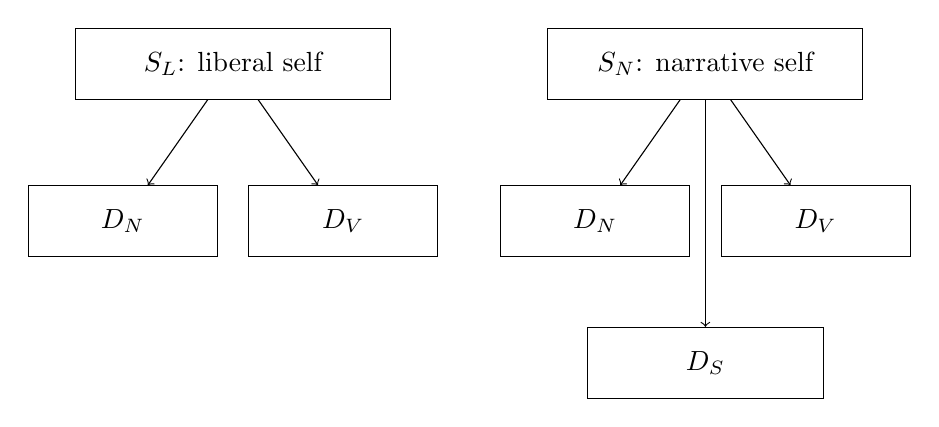
\begin{tikzpicture}[x=1cm,y=1cm]
\node[draw, rectangle, minimum width=4cm, minimum height=0.9cm] (SL) at (-3,3) {$S_L$: liberal self};
\node[draw, rectangle, minimum width=4cm, minimum height=0.9cm] (SN) at (3,3) {$S_N$: narrative self};

\node[draw, rectangle, minimum width=2.4cm, minimum height=0.9cm] (DN1) at (-4.4,1) {$D_N$};
\node[draw, rectangle, minimum width=2.4cm, minimum height=0.9cm] (DV1) at (-1.6,1) {$D_V$};

\node[draw, rectangle, minimum width=2.4cm, minimum height=0.9cm] (DN2) at (1.6,1) {$D_N$};
\node[draw, rectangle, minimum width=2.4cm, minimum height=0.9cm] (DV2) at (4.4,1) {$D_V$};
\node[draw, rectangle, minimum width=3cm, minimum height=0.9cm] (DS2) at (3,-0.8) {$D_S$};

\draw[->] (SL) -- (DN1);
\draw[->] (SL) -- (DV1);

\draw[->] (SN) -- (DN2);
\draw[->] (SN) -- (DV2);
\draw[->] (SN) -- (DS2);
\end{tikzpicture}
\caption{The lecture's formal spine: is the liberal taxonomy of obligation exhaustive, or must we add a third class of obligations arising from membership and solidarity?}
\end{figure}

\paragraph{A worked derivation.}
The lecture's conceptual derivation runs in a short chain:
\begin{enumerate}
\item If the self is fundamentally unencumbered, then unchosen histories do not bind simply as such.
\item If unchosen histories do not bind, obligations must arise either universally or voluntarily.
\item Hence the liberal equation \(D_N + D_V\).
\item If, however, the self is partly constituted by inherited memberships, then some obligations may arise neither from universality nor from consent.
\item Hence the communitarian extension \(D_N + D_V + D_S\).
\end{enumerate}

\subsection{Question \& Answer}

\paragraph{Question.} Is there a third category of obligation beyond universal duty and consent?

\paragraph{Answer.} Sandel's answer at this stage is not yet a final yes. It is rather that this is the exact question the lecture has earned. The communitarian position is not merely a feeling about loyalty; it is the claim that the liberal taxonomy omits a distinct class of obligations whose force comes from membership itself.

\section{Test Cases of Membership}

The lecture now turns to examples, and the order matters. Sandel begins with family, because the intuitions are strongest there, then moves outward into political community and patriotism. The point is to test whether \(D_S\) names a real moral phenomenon.

The first case is the drowning child. If one drowning child is mine and the other a stranger's, must I flip a coin? Sandel's point is that many of us would think there is something morally obtuse about the demand for strict impartiality here. The second case is even sharper, because the child does not choose his parents. If one aged parent is mine and the other is a stranger's, why does it seem morally intelligible that my obligation should fall more heavily on my own parent?

Schematically, the dispute over such cases may be written as
\begin{align}
\mathcal{O}_{\text{aged parent}} &\in \{D_V,\text{reciprocity}\} \quad \text{on the liberal reduction}, \\
\mathcal{O}_{\text{aged parent}} &= D_S \quad \text{on the communitarian reading}.
\end{align}

The political examples extend the same pressure. The French resistance pilot refuses to bomb his own village, not because the target is less important strategically, but because he cannot bring himself to bomb \emph{his people}. The Israeli airlift of Ethiopian Jews raises the same question in a different key: is the selective rescue a morally troubling partiality, or the proper recognition of a special obligation of solidarity?

From there Sandel widens the lens to patriotism. Why, if at all, should national boundaries matter morally? Why should need on one side of the river count differently from equal need on the other side? Here the lecture gives patriotism its strongest communitarian formulation:
\begin{equation}
\text{patriotism at least potentially a virtue} \Longrightarrow \text{an expression of the obligations of citizenship.}
\end{equation}

\subsection{Question \& Answer}

\paragraph{Question.} Why should family or country bind us more strongly than strangers if consent did not create the tie?

\paragraph{Answer.} The communitarian answer is that these ties help constitute the person who now reasons and acts. The tie is not merely an external fact; it is part of the identity from which practical judgment begins. The liberal answer, by contrast, tries to re-explain the same cases in terms of consent, reciprocity, or benefit. The rest of the lecture asks whether that reduction succeeds.

\section{Objections, the Mid-Lecture Reset, and the Harder Test}

Sandel now lets the room push back. The first objection is structural: if obligations of membership are real, then we inhabit too many communities at once, and their claims may conflict. That produces two rival ordering proposals, each of which the lecture treats as unstable:
\begin{align}
\text{most universal community} &\stackrel{?}{>} \text{more particular communities}, \\
\text{family} &\stackrel{?}{>} \text{town} \stackrel{?}{>} \text{country} \stackrel{?}{>} \text{humanity}.
\end{align}

The next objection is that patriotism may be only prejudice, a false narrative generated by arbitrary boundaries. The next is that apparent obligations of solidarity can be redescribed through reciprocity or benefit:
\begin{equation}
\text{consent} \lor \text{reciprocity} \stackrel{?}{\Longrightarrow} \text{all particular obligations}.
\end{equation}

The lecture then performs a genuine reset. Sandel announces that he now wants to consider the strongest objections to solidarity and membership. This is not repetition. It is a second pass in which the earlier objections are gathered into a tighter form: conflict of obligations, reduction to sentiment, reduction to reciprocity or consent, and the charge that communal obligation is a kind of collective selfishness.

A liberal reconstruction of the issue therefore looks like this:
\begin{enumerate}
\item Natural duties have priority over all local attachments.
\item Particular attachments are permissible if chosen.
\item They are also permissible if they do not violate universal duties.
\item But there is no need to posit a nonvoluntary moral category beyond these.
\end{enumerate}

What follows is Sandel's search for a more difficult case. It is not enough for defenders of community to cite instances where loyalty merely coincides with justice. They need a case where loyalty competes with universal moral claim and still seems to retain moral weight.

That is why the lecture turns to Dan, Billy Bulger, and Robert E. Lee. Dan will not report a cheating roommate. Billy Bulger refuses to help authorities catch his fugitive brother. Lee refuses to fight against Virginia even while opposing secession and while recognizing the magnitude of the Union cause. These are not safe examples. They are chosen precisely because the communitarian claim will either survive here or collapse.

\subsection{Question \& Answer}

\paragraph{Question.} Can loyalty ever compete with universal moral claims without collapsing into mere sentiment or wrongdoing?

\paragraph{Answer.} Sandel does not say simply that loyalty wins. His point is narrower and more difficult: in these cases loyalty appears to be more than sentiment. Even where the act may be wrong, there can still be something morally intelligible, perhaps even admirable, in the pull of loyalty. That is the strongest form of the communitarian challenge.

\paragraph{A worked classification.}
The lecture's harder cases can be sorted schematically:
\begin{enumerate}
\item Dan's case: loyalty to roommate seems to compete with truth-telling and fairness.
\item Billy Bulger's case: brotherly loyalty seems to compete with civic and legal responsibility.
\item Lee's case: loyalty to Virginia seems to compete with loyalty to Union and opposition to slavery.
\item Therefore the live question is not whether a choice must be made, but whether loyalty itself has independent moral weight in making it.
\end{enumerate}

\section{Justice and Social Meanings}

After the long exchange over obligation, the lecture widens once more. Suppose the communitarian challenge is right. Suppose the right cannot be detached from the good. Does it then follow that justice is bound to the shared understandings of each community?

Sandel introduces Walzer at this point as the strongest formulation of that possibility:
\begin{align}
\text{justice} &= \text{relative to social meanings}, \\
\text{just society} &= \text{faithfulness to the shared understandings of its members}.
\end{align}

This is the last formal move of the chapter, and it is deliberately risky. If justice is tied to communal meanings, then it gains historical depth and social embeddedness; but it also seems in danger of becoming convention-bound. We can summarize the worry the lecture now raises:
\begin{align}
\text{justice tied to shared meanings} &\Longrightarrow \text{conventionalism?} \\
\text{tradition} + \text{situated identity} &\not\Longrightarrow \text{justice}.
\end{align}

That final inequality is not offered as a theorem proved once and for all. It is an open pressure point. Sandel runs the clip from \emph{Eyes on the Prize} in order to show that defenders of segregation can also speak the language of tradition, situated identity, and shared understanding. If those appeals are enough, then the communitarian move threatens to justify what it set out to criticize.

\subsection{Question \& Answer}

\paragraph{Question.} If justice follows shared social meanings, what prevents convention from ratifying injustice?

\paragraph{Answer.} The lecture does not yet settle the issue. That is the point of the ending. Sandel closes by forcing the question into view: either communal meanings are not enough, or they must be interpreted in a way that can distinguish morally illuminating traditions from corrupt ones. The next step must therefore ask whether justice can remain socially situated without becoming hostage to whatever a community happens, at a given time, to honor.

\section{Summary}

We began with a contrast between Aristotle and Kant, but the lecture's real center lies one step later, in the question of what kind of self each view presupposes. From the unencumbered self came the liberal taxonomy \(D_N + D_V\); from the narrative self came the communitarian challenge that a third class, \(D_S\), is needed if we are to make sense of loyalty, membership, and solidarity. Sandel then tested that challenge through family, patriotism, and a series of difficult cases in which loyalty seems to compete with universal duty. The closing turn to Walzer shows what is at stake if the communitarian challenge is accepted too quickly: justice may gain social depth, but it may also seem to collapse into convention. The chapter therefore ends where the lecture ends, not with a resolution, but with a more exact question.